\documentclass{article}
\usepackage{graphicx}
\usepackage{amsmath}
\usepackage{hyperref}
\usepackage[margin=1in]{geometry}
\usepackage{enumerate} 

\title{CFD Course Report - Week 12}
\author{Your Name}
\date{\today}

\begin{document}

\maketitle

\begin{abstract}
This report summarizes the computational fluid dynamics (CFD) simulations and analyses conducted during week 12 of the course.
\end{abstract}

\newpage
\section{Task 1: Elementary Vector Calculus}
 
\subsection{Gradient of a scalar $\phi$:}
    \begin{equation}
        grad(\phi) = \nabla \phi = \frac{\partial \phi}{\partial x_i} = \left( \frac{\partial \phi}{\partial x}, \frac{\partial \phi}{\partial y}, \frac{\partial \phi}{\partial z} \right)
    \end{equation}
\subsection{Divergence of the velocity vector $\vec{u}$:}
    \begin{equation}
        div(\vec{u}) = \nabla \cdot \vec{u} = \frac{\partial u_i}{\partial x_i} = \frac{\partial u}{\partial x} + \frac{\partial v}{\partial y} + \frac{\partial w}{\partial z}
    \end{equation}
\subsection{Curl of the velocity vector (vorticity):}
    \begin{equation}
        rot(\vec{u}) = \nabla \times \vec{u} = 
        \begin{vmatrix}
        \hat{i} & \hat{j} & \hat{k} \\
        \frac{\partial}{\partial x} & \frac{\partial}{\partial y} & \frac{\partial}{\partial z} \\
        u & v & w
        \end{vmatrix}
    = \left( \frac{\partial w}{\partial y} - \frac{\partial v}{\partial z}, \frac{\partial u}{\partial z} - \frac{\partial w}{\partial x}, \frac{\partial v}{\partial x} - \frac{\partial u}{\partial y} \right)
    \end{equation}
\subsection{Material derivative of a scalar:}
    \begin{equation}
        \frac{D\phi}{Dt} = \frac{\partial \phi}{\partial t} + (\vec{u} \cdot \nabla) \phi = \frac{\partial \phi}{\partial t} + u \frac{\partial \phi}{\partial x} + v \frac{\partial \phi}{\partial y} + w \frac{\partial \phi}{\partial z}
    \end{equation}
\subsection{Material derivative of the velocity vector:}
    \begin{equation}
        \begin{aligned}
        \frac{D\vec{u}}{Dt} &= \frac{\partial \vec{u}}{\partial t} + (\vec{u} \cdot \nabla) \vec{u} \\
        &= \left(\frac{\partial u}{\partial t}, \frac{\partial v}{\partial t}, \frac{\partial w}{\partial t}\right) + \left(\frac{\partial u}{\partial x} + \frac{\partial v}{\partial y} + \frac{\partial w}{\partial z}\right) \left(u, v, z\right) \\
        &= \left(\frac{\partial u}{\partial t}, \frac{\partial v}{\partial t}, \frac{\partial w}{\partial t}\right) + \frac{\partial u_i}{\partial x_i} \left(u, v, z\right)
        \end{aligned}
    \end{equation}
\subsection{Rate-of-strain-tensor:}
    \begin{equation}
        S = \frac{1}{2} \left(\nabla \vec{u} + (\nabla \vec{u})^T\right) = \frac{1}{2} \begin{pmatrix} 
            2 \frac{\partial u}{\partial x} & \frac{\partial u}{\partial y} + \frac{\partial v}{\partial x} & \frac{\partial u}{\partial z} + \frac{\partial w}{\partial x} \\
            \frac{\partial v}{\partial x} + \frac{\partial u}{\partial y} & 2 \frac{\partial v}{\partial y} & \frac{\partial v}{\partial z} + \frac{\partial w}{\partial y} \\
            \frac{\partial w}{\partial x} + \frac{\partial u}{\partial z} & \frac{\partial w}{\partial y} + \frac{\partial v}{\partial z} & 2 \frac{\partial w}{\partial z}
            \end{pmatrix}
    \end{equation}
\subsection{Divergence of the rate-of-strain tensor:}
    \begin{equation}
        \begin{aligned}
        \nabla \cdot \mathbf{S} &= \frac{\partial S}{\partial x_i} = \frac{1}{2} \left(\frac{\partial}{\partial x}, \frac{\partial}{\partial y}, \frac{\partial}{\partial z}\right) \begin{pmatrix} 
        2 \frac{\partial u}{\partial x} & \frac{\partial u}{\partial y} + \frac{\partial v}{\partial x} & \frac{\partial u}{\partial z} + \frac{\partial w}{\partial x} \\
        \frac{\partial v}{\partial x} + \frac{\partial u}{\partial y} & 2 \frac{\partial v}{\partial y} & \frac{\partial v}{\partial z} + \frac{\partial w}{\partial y} \\
        \frac{\partial w}{\partial x} + \frac{\partial u}{\partial z} & \frac{\partial w}{\partial y} + \frac{\partial v}{\partial z} & 2 \frac{\partial w}{\partial z}
        \end{pmatrix} \\
        &= \frac{1}{2}\left(2\frac{\partial^2 u}{\partial x^2} + \frac{\partial^2 v}{\partial x \partial y} + \frac{\partial^2 u}{\partial y^2} + \frac{\partial^2 w}{\partial x \partial z} + \frac{\partial^2 u}{\partial z^2}, \right. \\
        &\quad \left. \frac{\partial^2 u}{\partial y^2} + \frac{\partial^2 v}{\partial x \partial y} + 2 \frac{\partial^2 v}{\partial y^2} + \frac{\partial^2 w}{\partial y^2} + \frac{\partial^2 v}{\partial y \partial z}, \right. \\
        &\quad \left. \frac{\partial^2 u}{\partial x \partial z} + \frac{\partial^2 w}{\partial x^2} + \frac{\partial^2 v}{\partial x \partial z} + \frac{\partial^2 w}{\partial y^2} + 2 \frac{\partial^2 w}{\partial z^2}\right)
        \end{aligned}
        \end{equation}


\newpage
\section{Task 2: Global versus local rotation}

\subsection{Sketch of the flows:}
\subsubsection*{Line vortex flow: \textnormal{$\vec{u} = [u_r, u_\theta, u_z] = \left[0, -\frac{\alpha}{r}, 0\right]$ }}
\begin{figure}[h!]
    \centering
    \begin{tabular}{cc}
        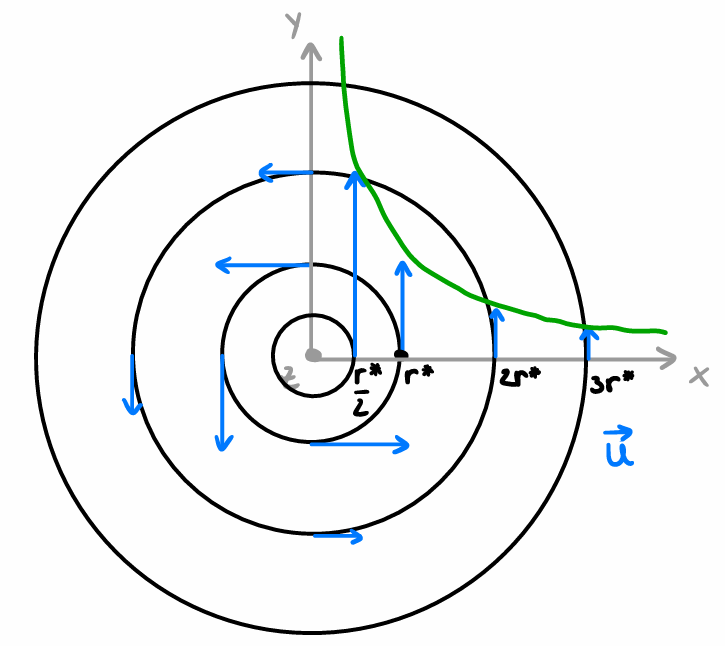
\includegraphics[width=0.20\textwidth]{imm_1.1.png} &
        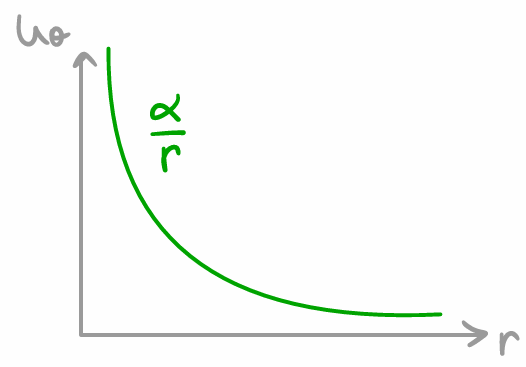
\includegraphics[width=0.20\textwidth]{imm_1.2.png}
    \end{tabular}
    \caption{Line vortex flow}
    \label{fig:mie_immagini}
\end{figure}
\subsubsection*{Plane shear flow: \textnormal{$\vec{u} = [u, v, w] = \left[\beta y, -0, 0\right]$}} 
\begin{figure}[h!]
    \centering
    \begin{tabular}{cc}
        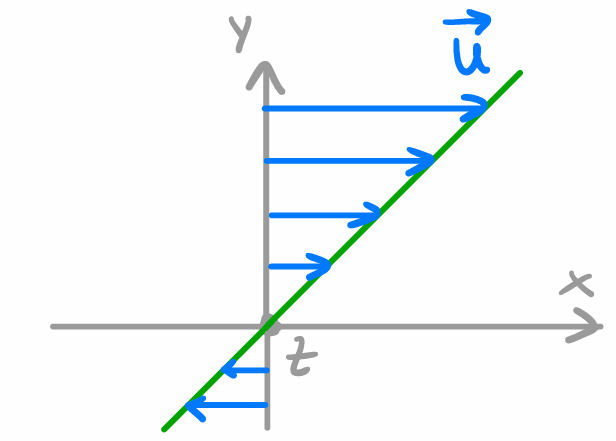
\includegraphics[width=0.20\textwidth]{imm_2.1.png} &
        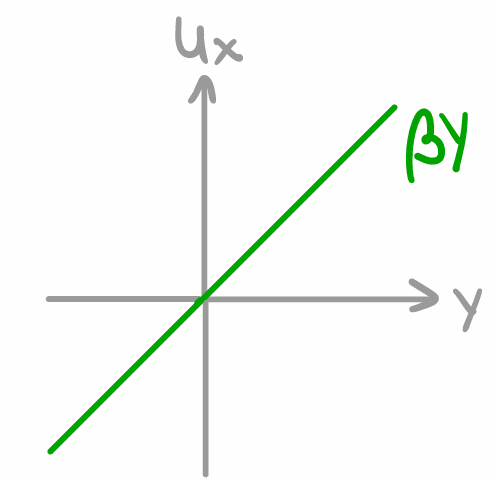
\includegraphics[width=0.20\textwidth]{imm_2.2.png}
    \end{tabular}
    \caption{Plane shear flow}
    \label{fig:mie_immagini}
\end{figure}
\subsubsection*{Flow between rotating cylinders: \textnormal{$\vec{u} = [u_r, u_\theta, u_z] = \left[0, Ar + \frac{B}{r}, 0\right]$}} 
\begin{figure}[h!]
    \centering
    \begin{tabular}{cc}
        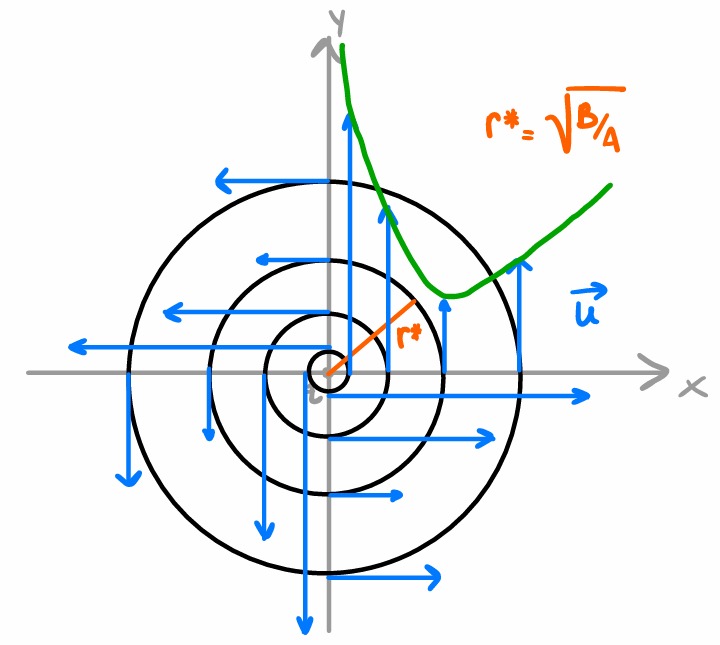
\includegraphics[width=0.20\textwidth]{imm_3.1.png} &
        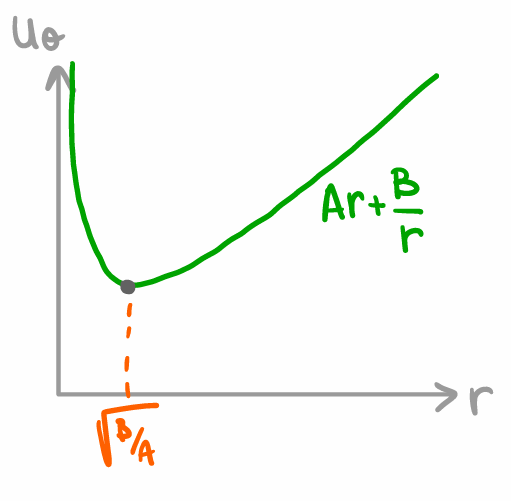
\includegraphics[width=0.20\textwidth]{imm_3.2.png}
    \end{tabular}
    \caption{Flow between rotating cylinders}
    \label{fig:mie_immagini}
\end{figure}


\subsection{Local and global rotations:}
To verify wheter a flow features a local/global rotation we need to compute its vorticity, which is a vector quantity defined as $\vec{\omega} = \nabla \times \mathbf{u}$.
\subsubsection*{Line vortex flow:}
For this specific flow we have that the vorticity vector is $\vec{\omega} = [0, 0, 0]$, so this flow does not show a local nor a global rotation since the vorticity is the null vector.
\subsubsection*{Plane shear flow:}
Making usage of the previously delined formula for the vorticity, we find that $\vec{\omega}  = \left[0, 0, -\beta\right]$ which indicates that we have a shear-induced rotation around the $z$-axis. Also this flow does not feature a global rotation because it is characterized by a velocity gradient in the $y$-direction (shear) rather than a circular motion and this causes fluid elements to rotate locally due to the velocity differences at different $y$-positions, but there is no coordinated or structured rotation of the entire flow field. The flow is linear, not circular, so it doesn't exhibit global rotation. 
\subsubsection*{Flow between rotating cylinders:}
As in the former cases we compute the vorticity: $\vec{\omega} = [0, 0, 2A]$. Also the third flow exibits a local rotation due to the non-zero vorticiy, but unlike the previous cases the rotating cylinders create a structured and circular flow with a consistent rotational effect through the domain. 

In all three cases, we could have reached similar conclusions by observing the graphs shown above.


\newpage
\section{Task 5: Simplifications of Navier-Stokes Equations}

\end{document}
